\begin{ZhChapter}

\chapter{Methodology}
In this session, we will introduce the S2GE-NIDS (structured semantics and generation embedded network intrusion detection system) architecture and details its operational workflow, clearly delineating each step from semantic tokenization through anomaly detection and decision-making processes.
\section{Architecture} %Chapter 3.1
S2GE-NiDS is presented as Figure \ref{fig: Architecture} including preprocess model, embedding model, and Mahalanobis model.

\begin{figure*}[htbp]
    \centering
    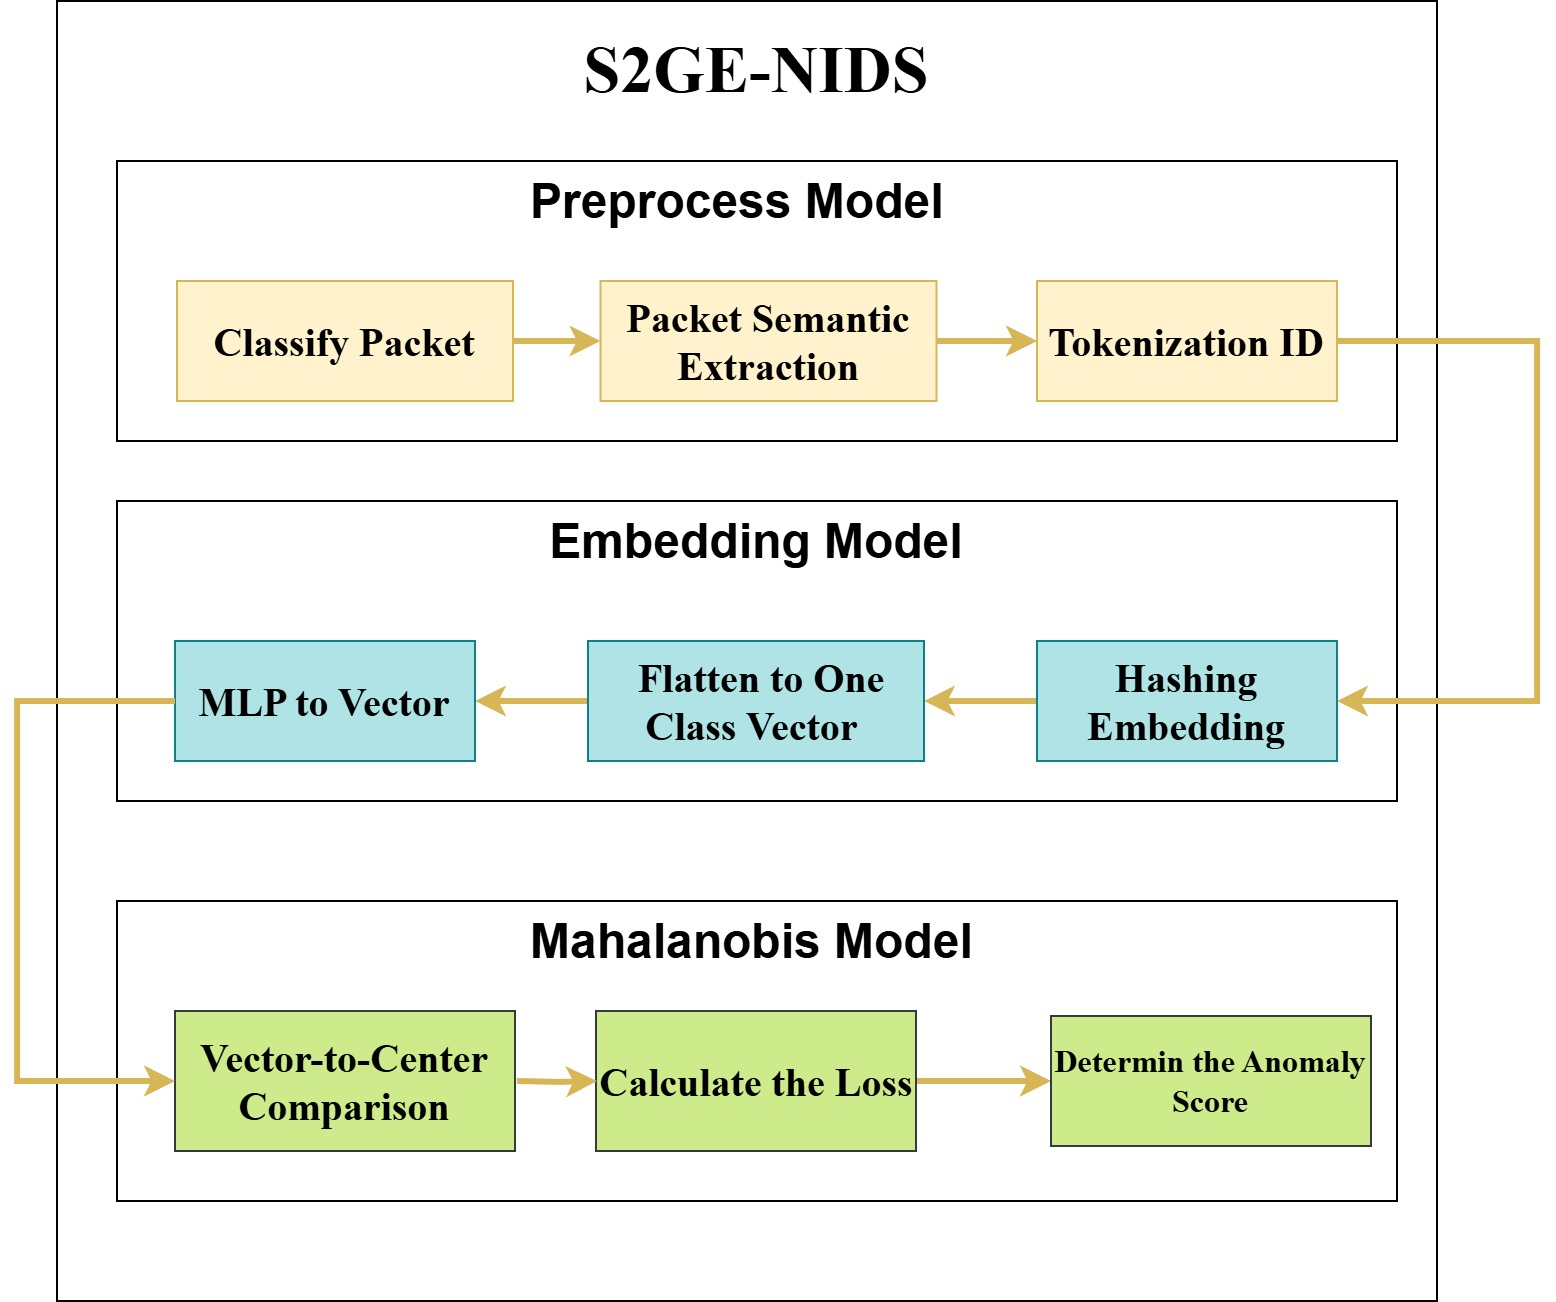
\includegraphics[width = 0.75\textwidth]{image/Flow.jpg}
    \caption{Architecture of S2GE-NIDS}
    \label{fig: Architecture}
\end{figure*}

During the preprocessing stage, relevant features are first extracted from network data packets and transformed into a combination of textual and numerical tokens. To prevent duplication and ensure a more uniform distribution within the embedding space, the model applies the non-encrypted MurmurHash3 function to encode each token.

To further mitigate the risk of hash collisions, a modulo operation is performed on the resulting hash values, which are then used to index into the embedding table. This strategy reduces the likelihood of different tokens being mapped to the same location, thereby enhancing both the accuracy and efficiency of the embedding process.

Next, the individual embedding vectors corresponding to each feature are concatenated into a single one-dimensional vector. This flattened vector is fed into a multi-layer perceptron (MLP) model, which transforms it into a compact semantic representation.

Finally, in the Mahalanobis distance evaluation phase, the semantic vector is compared to a predefined center point in the learned semantic space. If the computed distance exceeds a specified threshold, the sample is flagged as an anomaly. Evaluation metrics such as the F1 score are then used to quantify detection performance.

\subsection{Preprocess Model}
In the preprocessing phase, we will do the following process as data file selection and filtering, feature extraction, and tokenization. These steps are designed to transform raw network traffic into structured representations suitable for semantic embedding and anomaly detection.

\subsubsection{Classify Data Packet}

The first step in the preprocessing pipeline involves selecting and filtering the data files to ensure suitability for subsequent analysis. In this study, network traffic is collected and stored in the Comma-Separated Values (CSV) format—a widely adopted and flexible tabular data structure. CSV files are particularly well-suited for structured data representation due to their ease of parsing, compact storage, and seamless integration with mainstream data analysis libraries such as pandas and NumPy in Python.During this stage, only those CSV files containing the required packet-level features are retained, while incomplete, irrelevant, or malformed files are systematically excluded.

\subsubsection{Packet Semantic Extraction}

After the dataset is cleaned and organized, the first step is to extract meaningful features from the network packet records to effectively characterize the behavior of each packet. Prior research has demonstrated that certain fields are particularly effective in identifying anomalous or malicious patterns in network traffic.

In this study, we focus on a set of key attributes that are widely adopted in anomaly detection systems, including:Flow Duration, Header Length, Protocol Type, Duration, Rate, fin flag number and syn flag number. These features are highly relevant in distinguishing between normal and abnormal connections. The dataset includes a wide variety of network attack types, such as \texttt{DDoS-RSTFINFlood}, \texttt{DoS-TCP\_Flood}, and \texttt{DDoS-ICMP\_Flood}, making it rich and diverse for anomaly detection research.

In practical implementation, we employ Python-based tools to load each \texttt{.csv} file and extract the selected features as the primary input to the proposed S2GE-NIDS model. By focusing exclusively on these critical fields, the input data becomes cleaner and more interpretable, thereby enhancing the effectiveness and efficiency of the anomaly detection pipeline.


\subsubsection{Tokenization ID}
After the relevant features have been extracted, the next step is to perform tokenization, which converts structured data into a format suitable for semantic embedding. Each data entry consists of multiple fields—such as \texttt{Destination Port}, \texttt{Protocol}, and \texttt{SrcIP}—that represent different aspects of network behavior.

Tokenization is achieved by concatenating each field name with its corresponding value to form a unique string representation. This composite token serves as the semantic unit used in downstream embedding processes. For example, tokens follow the format \textit{"field name + field value"}, as illustrated in Table~\ref{tab:token_example}.


\begin{table*}[htbp]
    \centering
    \caption{Example of Tokenized Input Fields} \label{tab:token_example}
    \makebox[\linewidth][c]{
        \renewcommand\arraystretch{1.2}{
            \begin{tabular}{| l | l |}
                \hline
                \textbf{Field Name} & \textbf{Field Value} \\
                \hline
                Header Length       & 54                   \\
                Flow Duration       & 0.32817              \\
                Protocol Type       & TCP                  \\
                \hline
            \end{tabular}
        }}
\end{table*}



\subsection{Embedding Model}
To mitigate redundancy in text features during the embedding process, we employ a lightweight, non-cryptographic hash function—MurmurHash3. This function ensures that input tokens are more uniformly distributed across the embedding space, thus reducing overrepresentation in specific regions. To further minimize the probability of hash collisions—i.e., multiple tokens being mapped to the same position—we apply a modulo operation to the resulting hash values. This yields a deterministic index used to locate or store each feature vector within a fixed-size embedding table, enhancing both the accuracy and efficiency of the overall embedding process.

Once all relevant token embeddings are retrieved, their vectors are concatenated into a single flattened, one-dimensional feature vector. This unified representation is then fed into a multi-layer perceptron (MLP), which learns high-level semantic abstractions and generates a compact semantic feature vector. The subsequent subsections provide detailed descriptions of the hash embedding mechanism, the flattening procedure, and the structure of the MLP used for semantic encoding.

\subsubsection{Hash Embedding}
Hash embedding is a lightweight vectorization technique that utilizes non-cryptographic hashing to encode tokenized field-value pairs into fixed-size, trainable embeddings~\cite{weinberger2009feature}. In this study, we adopt the MurmurHash3 algorithm—an efficient and widely used hash function—to map each token to a specific position in the embedding table. Its advantages include fast computation, uniform distribution, and language-independent implementation, which make it well-suited for scalable anomaly detection in IoT environments~\cite{appleby2011murmurhash}.

To determine the target index for each token, we apply a modulo operation to the hash value using the smallest three-digit prime number, 1024. This approach distributes tokens more evenly within the embedding space and reduces collision rates. For example, the token generated from the field name \texttt{Protocol Type} may yield a MurmurHash3 value of 4283257230. Applying \texttt{4283257230 mod 1024} results in 56. If the associated port number (e.g., TCP) is similarly hashed and gives a value with mod 1024 result of 7, these indices (row 7, column 56) are used to locate the corresponding vector in the embedding table.

Each embedding vector is initially randomized and refined during training. For instance, an example 8-dimensional vector might be:

Table~\ref{tab: EmbeddingTable} illustrates a subset of the embedding table used in our model. Each row corresponds to a unique index obtained by applying the MurmurHash3 function and modulo operation to a specific token (e.g., \texttt{Header\_Length\_54}). The resulting index is used to retrieve an 8-dimensional embedding vector, which captures semantic properties of the original field-value token. These vectors are subsequently concatenated and passed into the MLP encoder to generate a semantic representation.

\begin{table*}[htbp]
\centering
\caption{Embedding Table} \label{tab: EmbeddingTable}
\makebox[\linewidth][c]{
    \renewcommand\arraystretch{1.2}{
        \begin{tabular}{| l | c | c |}
        \hline
        Number & Vector \\
        \hline
        459 \& -0.982, -0.301, -0.555,  2.061,  0.045, -0.618, -0.786,  0.573
        \hline
        44 \& 0.120,  1.202, -0.337, -0.982,  0.847,  0.110,  0.305, -0.499
        \hline
        984 \& -0.024,  0.494,  0.754, -0.780, -1.002,  0.069, -0.520, -1.336
        \hline
        \end {tabular}
    }}
\end {table*}



These vectors are later concatenated and passed to the MLP model for further semantic encoding.

In this study, we leverage the concept of \textit{Feature Hashing}~\cite{weinberger2009feature} to construct a two-dimensional embedding table that semantically encodes discrete field-value tokens. The embedding table is defined with dimensions $P \times D$, where $P = 1024$ is a selected prime number intended to reduce the probability of hash collisions, and $D = 8$ represents the dimensionality of the embedding vectors.

Each categorical input token (e.g., \texttt{Protocol:TCP}) is converted into an embedding through a dual-stage hashing process implemented with the MurmurHash3 algorithm:

\begin{itemize}
    \item \textbf{Stage 1: Field Hashing.} The field name (e.g., \texttt{Protocol}) is hashed and mapped to a row index:

          \begin{equation}
              \text{row} = \text{MurmurHash3}(\text{field}) \bmod P
              \label{eq:row_hash}
          \end{equation}

    \item \textbf{Stage 2: Value Hashing.} The field value (e.g., \texttt{TCP}) is independently hashed and mapped to a column index:

          \begin{equation}
              \text{col} = \text{MurmurHash3}(\text{value}) \bmod P
              \label{eq:col_hash}
          \end{equation}
\end{itemize}

Equations~\eqref{eq:row_hash} and~\eqref{eq:col_hash} are inspired by the Feature Hashing method proposed in~\cite{weinberger2009feature}, where we utilize MurmurHash3 as the underlying hash function~\cite{appleby2011murmurhash}.


This two-dimensional indexing scheme ensures that each field-value pair is assigned to a unique embedding vector in the table, while preserving sparsity and reducing memory consumption. By decoupling the field and value into separate hash functions, the design enhances semantic disentanglement and increases robustness against data sparsity and hash collisionsm ~\ref{fig:hashembedding}.


\begin{figure*}[htbp]
    \centering
    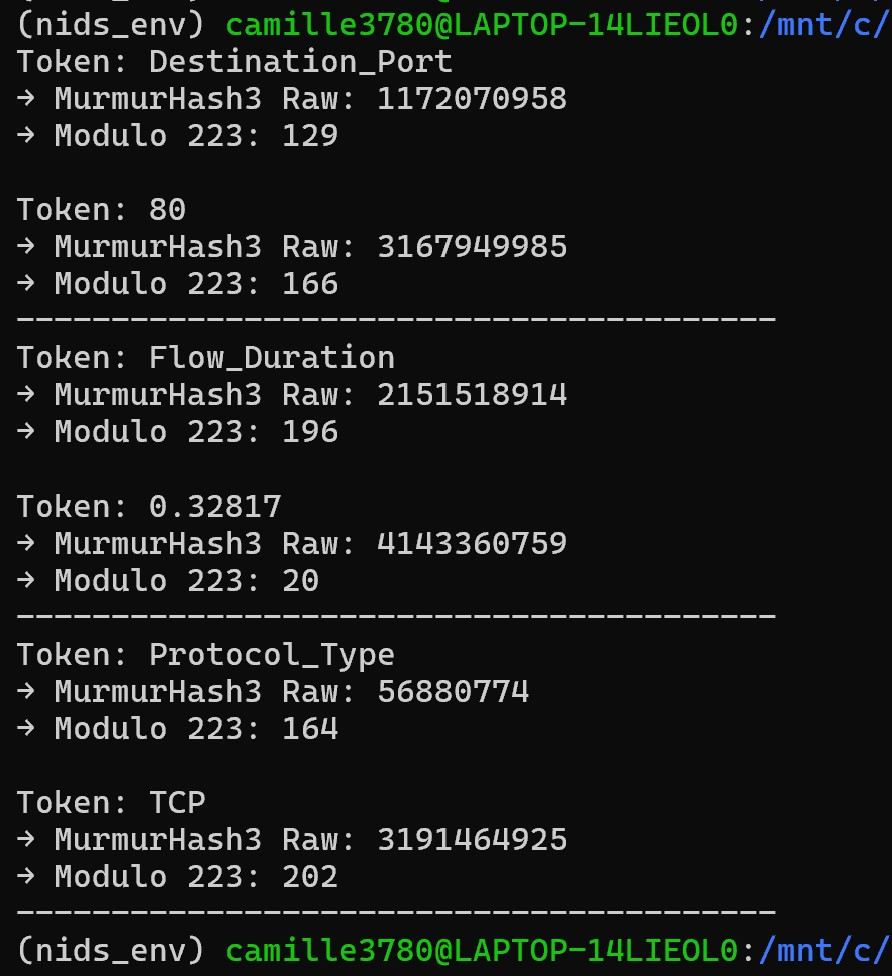
\includegraphics[width = 1\textwidth]{image/2025-06-30 002218.jpg}
    \caption{FlowChart for Efficiency-based GP}
    \label{fig: hashembedding}
\end{figure*}




\subsubsection{Flatten}
Flatten will string the tokenized data into a single vector through the vectors after the embedding column. For example, Header Length 54 is [-0.982, -0.301, -0.555,  2.061,  0.045, -0.618, -0.786,  0.573] and Protocol TCP tokeniz to [0.120,  1.202, -0.337, -0.982,  0.847,  0.110,  0.305, -0.499] ,Flow Duration 0.32817 [-0.024,  0.494,  0.754, -0.780, -1.002,  0.069, -0.520, -1.336], then the final flatten will be [-0.982, -0.301, -0.555, 2.061, 0.045, -0.618, -0.786, 0.573, -0.024, 0.494, 0.754, -0.78, -1.002, 0.069, -0.52, -1.336, -1.042, -0.116, 0.542, -0.987, 1.001, 0.086, 0.699, -0.903]


\subsubsection{MLP}
\section{Related Work: Multi-Layer Perceptron in IoT Anomaly Detection}

The Multi-Layer Perceptron (MLP) is one of the foundational deep learning architectures, widely used in classification and anomaly detection tasks due to its simplicity and capability to model non-linear decision boundaries. In the context of IoT network traffic analysis, MLP has been adopted as a lightweight yet powerful model for detecting abnormal behaviors across various device and protocol types.

\citet{shone2018deep} introduced a hybrid deep learning approach combining a stacked autoencoder with an MLP classifier to detect network intrusions. Their model was evaluated on the NSL-KDD dataset, achieving an accuracy of 85.42\% and demonstrating superior performance over classical ML algorithms such as decision trees and SVM.

Similarly, \citet{rahman2020deep} applied a pure MLP-based architecture for anomaly detection in the BoT-IoT dataset. The network consisted of three hidden layers with ReLU activation and dropout regularization. The results showed that MLP achieved over 98.5\% detection accuracy and maintained a false positive rate below 1\%, outperforming traditional algorithms such as KNN and Naive Bayes.

\citet{javaid2016deep} further explored MLP in a deep learning pipeline tailored for IoT environments. They emphasized the importance of feature normalization and used a softmax output layer for multi-class classification. Their experiments on KDDCup'99 and UNSW-NB15 datasets revealed that MLP models trained on optimized features could achieve both high recall and precision in detecting diverse attack types, including DoS, probing, and user-to-root exploits.

Despite its effectiveness, MLP has certain limitations. It lacks spatial or temporal awareness, making it less suitable for sequential data unless combined with other architectures (e.g., LSTM or CNN). However, for static, tabular representations of network flows, MLP remains a competitive choice due to its fast inference and low memory footprint, which are critical in real-time IoT security deployments.

These findings suggest that MLP can serve as a strong baseline model in IoT anomaly detection pipelines, especially when combined with proper feature engineering and regularization techniques.

Given an input vector $\mathbf{x} \in \mathbb{R}^d$, the computation through an MLP with $L$ hidden layers can be described as:

\begin{equation}
    \mathbf{h}^{(1)} = \sigma\left( \mathbf{W}^{(1)} \mathbf{x} + \mathbf{b}^{(1)} \right)
    \label{eq:mlp_layer1}
\end{equation}

\begin{equation}
    \mathbf{h}^{(l)} = \sigma\left( \mathbf{W}^{(l)} \mathbf{h}^{(l-1)} + \mathbf{b}^{(l)} \right), \quad \text{for } l=2, \dots, L
    \label{eq:mlp_hidden}
\end{equation}

\begin{equation}
    \hat{\mathbf{y}} = f\left( \mathbf{W}^{(L+1)} \mathbf{h}^{(L)} + \mathbf{b}^{(L+1)} \right)
    \label{eq:mlp_output}
\end{equation}

Where:
\begin{itemize}
    \item $\mathbf{W}^{(l)}$ and $\mathbf{b}^{(l)}$ are the weight matrix and bias vector of layer $l$
    \item $\sigma(\cdot)$ is a non-linear activation function (e.g., ReLU)
    \item $f(\cdot)$ is the output activation function (e.g., sigmoid or softmax)
    \item $\hat{\mathbf{y}}$ is the predicted output vector
\end{itemize}

\subsection{Activation Functions}

Common activation functions include:

\begin{itemize}
    \item \textbf{ReLU:} $\sigma(z) = \max(0, z)$
    \item \textbf{Sigmoid:} $\sigma(z) = \frac{1}{1 + e^{-z}}$
    \item \textbf{Tanh:} $\sigma(z) = \tanh(z) = \frac{e^z - e^{-z}}{e^z + e^{-z}}$
\end{itemize}

\subsection{Loss Functions}

For binary classification, the binary cross-entropy loss is used:

\begin{equation}
    \mathcal{L}_{\text{binary}} = - \frac{1}{N} \sum_{i=1}^{N} \left[ y_i \log(\hat{y}_i) + (1 - y_i) \log(1 - \hat{y}_i) \right]
    \label{eq:binary_loss}
\end{equation}

For multi-class classification with $C$ classes, the categorical cross-entropy is used:

\begin{equation}
    \mathcal{L}_{\text{categorical}} = - \frac{1}{N} \sum_{i=1}^{N} \sum_{c=1}^{C} y_{i,c} \log(\hat{y}_{i,c})
    \label{eq:categorical_loss}
\end{equation}

\subsection{Backpropagation and Gradient Computation}

Training is performed via gradient-based optimization (e.g., SGD, Adam), using backpropagation to compute gradients.

Gradient of loss with respect to weights in layer $l$:

\begin{equation}
    \frac{\partial \mathcal{L}}{\partial \mathbf{W}^{(l)}} = \delta^{(l)} \cdot \left( \mathbf{h}^{(l-1)} \right)^\top
    \label{eq:gradient_weight}
\end{equation}

Recursive definition of error term:

\begin{equation}
    \delta^{(l)} = \left( \mathbf{W}^{(l+1)\top} \delta^{(l+1)} \right) \circ \sigma'\left( \mathbf{z}^{(l)} \right)
    \label{eq:delta_recursive}
\end{equation}

Where $\circ$ denotes element-wise multiplication, and $\sigma'(\cdot)$ is the derivative of the activation function.


\subsection{Mahalanobis Distance Model}
In the final stage of the S2GE-NIDS framework, we apply a statistical distance-based method—\textbf{Mahalanobis Distance}—to evaluate whether an observed semantic vector deviates significantly from the expected distribution of normal traffic. This metric is particularly effective for high-dimensional anomaly detection, as it accounts for feature correlations and variance~\cite{de2000mahalanobis}.

Let $\mathbf{x} \in \mathbb{R}^n$ denote the semantic vector output from the MLP, and let $\boldsymbol{\mu}$ and $\boldsymbol{\Sigma}$ represent the mean vector and covariance matrix estimated from a subset of benign (normal) training data. The Mahalanobis distance is defined as:

This formulation enables the model to assess how far a sample deviates from the learned semantic center under multivariate normality assumptions. During inference, if $D_M(\mathbf{x})$ exceeds a predefined threshold $\tau$, the corresponding traffic instance is flagged as an anomaly.

We empirically determine $\tau$ using the distribution of distances in the training set, often by selecting a percentile threshold (e.g., 95th percentile). This thresholding strategy is advantageous in unsupervised or semi-supervised settings, where labeled anomaly samples may be scarce.

The integration of Mahalanobis scoring into our system introduces the benefits of model interpretability and statistical rigor, effectively enhancing the ability to detect subtle but semantically meaningful deviations in IoT network behavior.


\subsubsection{Vector-to-Center Comparison}
To enhance anomaly detection, S2GE-NIDS introduces a center loss mechanism. During training, all semantic vectors corresponding to ``normal'' samples are aggregated to calculate a center point $c$.

\begin{itemize}
    \item Taking into account the variability and correlation of each feature, the model can more accurately detect abnormal samples that are ``off-center''.
\end{itemize}

\begin{equation}
    D_M(z) = \sqrt{(z - c)^T \Sigma^{-1} (z - c)} \tag*{\makebox[3.8cm][r]{\cite{mahalanobis1936generalized}}}
    \label{eq:mahalanobis}
\end{equation}

$z$ is the semantic vector of the input sample, $c$ is the center vector of normal samples, and $\Sigma^{-1}$ is the inverse of the covariance matrix of the training data's embedding vectors.


\subsubsection{Calculate the Loss}
\begin{itemize}
    \item The loss is defined as:
\end{itemize}

\begin{equation}
    \mathcal{L} = \frac{1}{N} \sum_{i=1}^{N} \| z_i - c \|^2
    = \frac{1}{N} \sum_{i=1}^{N} \sum_{j=1}^{d} (z_{ij} - c_j)^2 \tag*{\makebox[3.8cm][r]{\cite{mlp2001universal}}}
    \label{eq:centerloss}
\end{equation}

$z_i \in \mathbb{R}^d$ is the embedding vector obtained after the $i$th input passes through the Semantic Encoder,
$c \in \mathbb{R}^d$ is the center point vector during training (center), and $N$ is the total number of samples.



\subsubsection{Determine the Anomaly Score}
After obtaining the semantic vector $z$ of each input data point through the MLP encoder, and computing the center point $c$ based on all normal training samples, the system evaluates how far each sample deviates from the normal data distribution using the Mahalanobis distance metric.

The Mahalanobis distance score $D_M(z)$, as defined in Equation ~\ref{eq:liu2020anomaly}, quantifies the distance between a sample's semantic representation $z$ and the center vector $c$, while accounting for the variance and covariance of the embedding space. This distance serves as the anomaly score for each sample.

\begin{equation}
    D_M(z) = \sqrt{(z - c)^T \Sigma^{-1} (z - c)} \tag*{\makebox[3.8cm][r]{\cite{de2000mahalanobis}}}
\end{equation}

To determine whether a sample is anomalous, we define a threshold $\tau$ based on the distribution of distances observed in the training data. A sample is classified as anomalous if its Mahalanobis distance exceeds this threshold:

\begin{equation}
    \text{Anomaly}(z) =
    \begin{cases}
        1 & \text{if } D_M(z) > \tau                                            \\
        0 & \text{otherwise} \tag*{\makebox[3.8cm][r]{\cite{mlp2001universal}}}
    \end{cases}
\end{equation}

Here, $\tau$ can be determined in several ways, such as:
\begin{itemize}
    \item Using the mean plus $k$ standard deviations from the training distribution (e.g., $\tau = \mu + k\sigma$).
    \item Setting $\tau$ based on a desired false-positive rate (e.g., the 95th percentile of $D_M(z)$ on normal samples).
\end{itemize}

This threshold-based mechanism enables the system to make binary decisions (normal vs. anomalous) while preserving the interpretability and statistical grounding of the anomaly scores. Additionally, ranked anomaly scores $D_M(z)$ can be used in top-$k$ selection scenarios for prioritizing the most suspicious samples in real-time applications.







\section{Flow} %Chapter 3.2
\subsection{Preprocess Model}
As shown in the figure \ref{fig:FlowChart}, the system receives the uploaded network packet data and checks if the data format matches the CSV (Comma-Separated Values) format. If the data is not in CSV format, the system will prompt the user to re-upload the data. In the next stage, the system cleans the data fields, including removing any missing or empty fields from the packets.
\begin{figure*}[htbp]
    \centering
    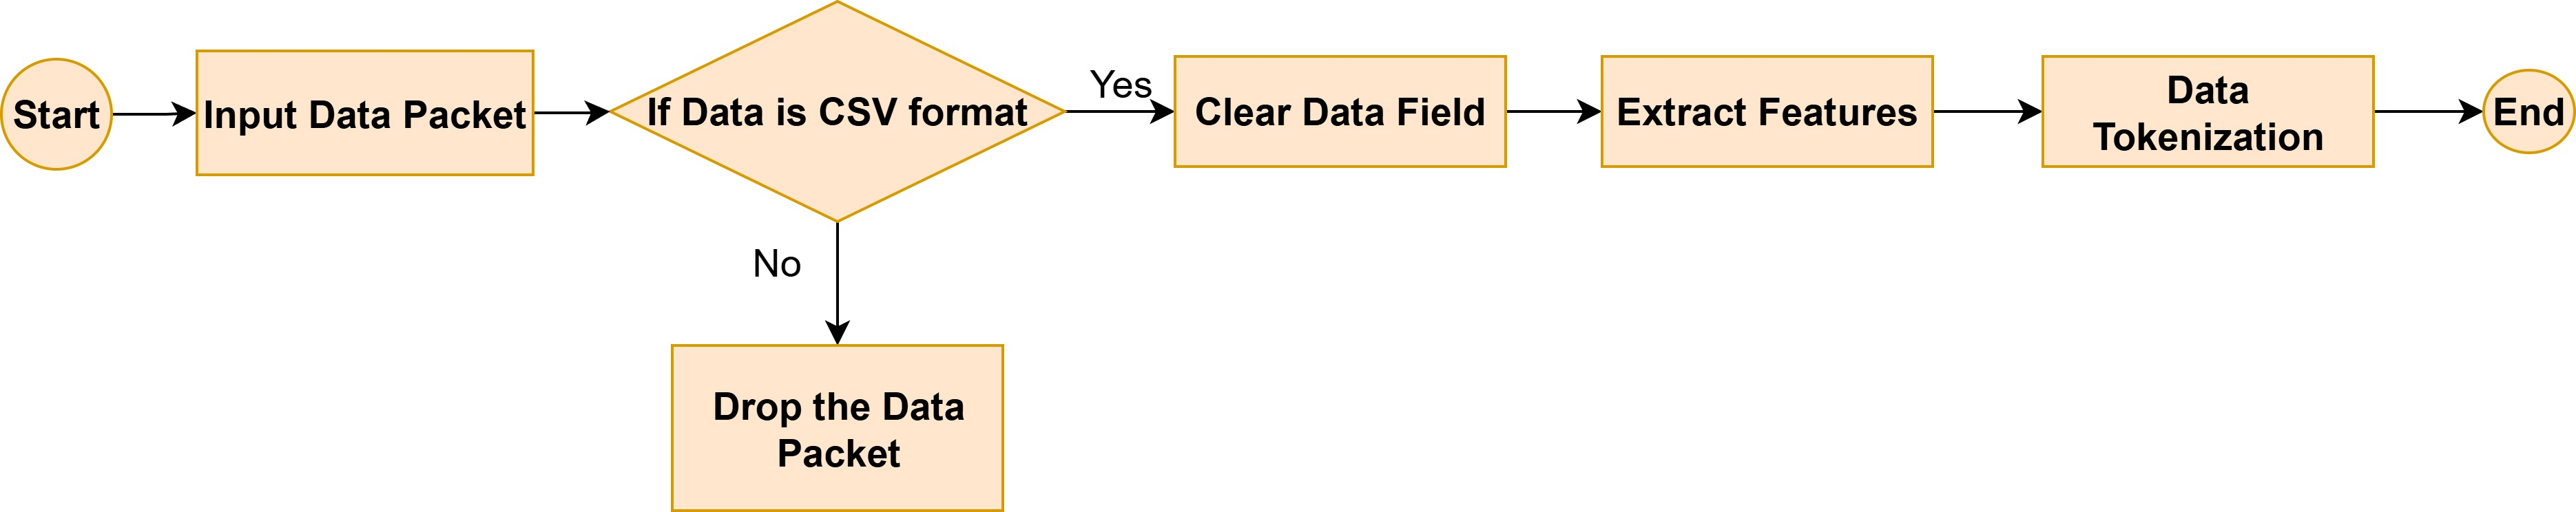
\includegraphics[width = 0.5\textwidth]{image/FlowChart.jpg}
    \caption{FlowChart for Preprocess Model}
    \label{fig:FlowChart}
\end{figure*}

Subsequently, specific fields related to common anomaly detection features are extracted, such as Destination Port, Protocol Type, and Source IP (SrcIP). These fields serve as important inputs for subsequent model analysis.

Finally, the field names and their respective values are combined into tokens---for instance, \texttt{Protocol\_TCP} or \texttt{Port\_80}---and fed into a semantic embedding model to be transformed into vectors for further processing.



\subsection{Implementation Procedure}
The system implementation is divided into several sequential stages, including: data preprocessing, feature transformation, semantic embedding, and anomaly detection. The detailed procedure is as follows:

\textbf{Step 1. Input Network Packet Data}
The raw data used in this study is stored in Comma-Separated Values (CSV) format. This format is chosen due to its ease of parsing and manageability. The dataset contains detailed information about various network packets.

\textbf{Step 2. Data Cleaning and Filtering}
After loading the dataset, the preprocessing phase is initiated. This phase includes data cleaning and filtering. The system removes missing values and clearly anomalous packet records to avoid introducing bias or errors in subsequent processing stages.

\textbf{Step 3. Feature Selection}
Based on insights from related research, specific key feature fields are selected from the raw packet data to serve as input for the model. These primarily include destination port, communication protocol, and source IP address. The selection is made based on the features’ effectiveness in distinguishing anomalous events.

\textbf{Step 4. Feature Tokenization}
To enhance the model’s ability to process both textual and numerical features, each feature field is combined with its corresponding value to form semantically meaningful tokens. For instance, a destination port of 80 is converted into the token “Port\_80”.


\begin{figure*}[htbp]
    \centering
    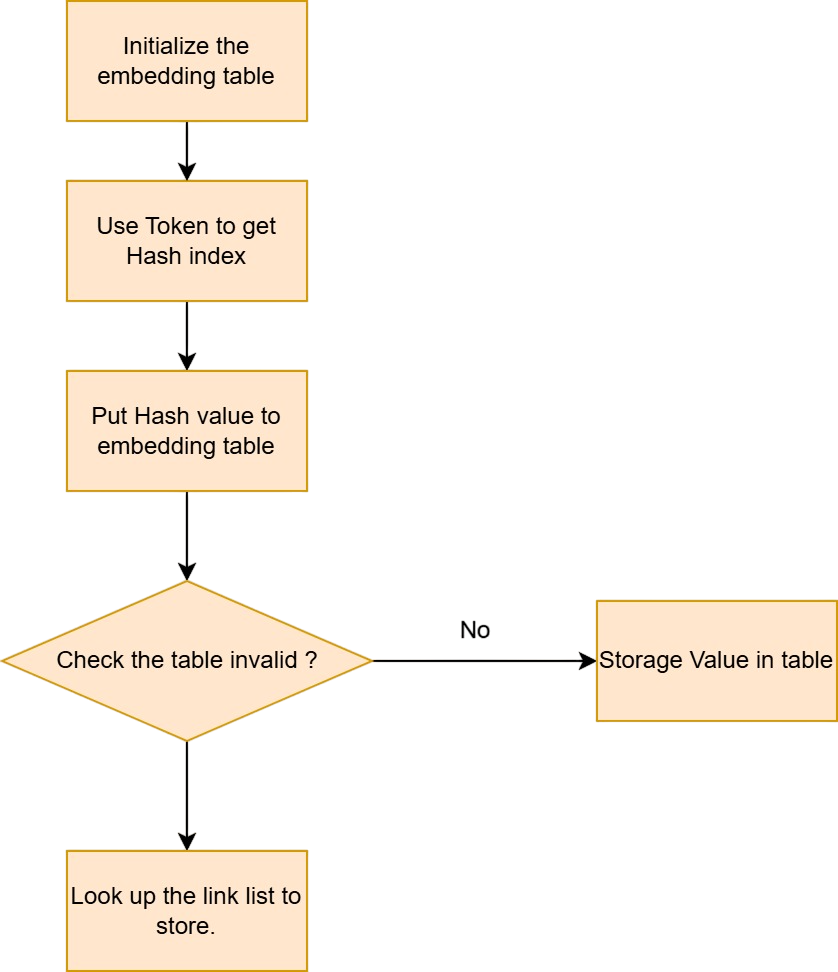
\includegraphics[width = 0.5\textwidth]{image/hashembedding.jpg}
    \caption{Hash Embedding for Embedding Model}
    \label{fig: HashEmbedding}
\end{figure*}

\textbf{Step 5. Feature Hash Mapping}
Since tokens often exhibit high redundancy and dimensionality, each token is passed through the MurmurHash3 hashing function (figure \ref{fig: HashEmbedding}) to generate a fixed-length hash value. This reduces dimensionality and ensures even distribution, thereby improving computational efficiency and mitigating potential collision issues.

\textbf{Step 6. Constructing the Embedding Table}
Each hashed token is assigned a randomly initialized embedding vector. These vectors are stored in an embedding table that maps discrete hash values into a continuous vector space, facilitating the generation of semantic representations.

\textbf{Step 7. Semantic Embedding}
All token vectors associated with a given packet are concatenated and flattened into a single vector, which is then passed through a Multi-Layer Perceptron (MLP) to perform nonlinear transformation. The output is a semantically enriched vector representation of the packet.

\textbf{Step 8. Establishing the Normal Sample Center Vector}
To enable effective anomaly detection, the system computes the mean vector of all semantic vectors derived from normal packets during the training phase. This average vector serves as the center representation of normal traffic and is denoted as $c$.

\textbf{Step 9. Anomaly Scoring via Mahalanobis Distance}
During the detection phase, the system calculates the Mahalanobis distance $D_M(z)$ between the semantic vector $z$ of each incoming packet and the normal center vector $c$. If the computed distance exceeds a predefined threshold, the packet is classified as anomalous.

This systematic implementation procedure enables accurate and efficient anomaly detection on network packet data.


\end{ZhChapter}